\documentclass{article}
\usepackage{graphicx} % Required for inserting images
\usepackage[left=4cm, right=4cm, top=4cm, bottom=4cm]{geometry}
\usepackage[T1]{fontenc}
\usepackage[polish]{babel}
\usepackage{amssymb}
\usepackage{url}
\usepackage{enumitem}
\usepackage{dirtree}
\usepackage[export]{adjustbox}
\usepackage{amsmath}
\usepackage{float}



\title{\Huge JIMP2 Projekt 2025 \\ {\huge Dokumentacja funkcjonalna - Java}}
\author{Michał Ludwiczak \\ GR3}
\date{29 kwietnia 2025}

\begin{document}

\maketitle

\tableofcontents



\section{Cel projektu}

    Celem projektu jest stworzenie aplikacji w języku Java, umożliwiającej podział grafu na określoną przez użytkownika liczbę części, z zachowaniem określonego lub domyślnego 10-procentowego marginesu różnicy liczby wierzchołków pomiędzy częściami. Domyślnie graf dzielony jest na dwie części. Celem podziału jest także minimalizacja liczby przeciętych krawędzi pomiędzy powstałymi częściami grafu. 
    Aplikacja będzie wyposażona w graficzny interfejs użytkownika wykonany w technologii Swing. Użytkownik będzie mógł wczytywać graf z pliku tekstowego lub binarnego, definiować liczbę części oraz margines podziału, a także zapisywać wynikowy graf wraz z danymi wejściowymi do pliku tekstowego lub binarnego. 
    Każda część grafu będzie prezentowana w interfejsie graficznym w odrębnym kolorze.
    
    \begin{figure}[H]
        \centering
        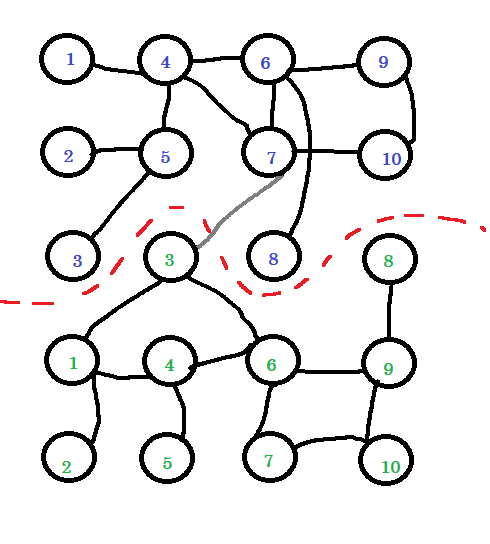
\includegraphics[width=0.75\linewidth]{img/graph.png}
        \caption{Przykładowy graf podzielony na 2 równe części}
        \label{fig:graph}
    \end{figure}



\section{Problem}

    Podział grafu na części w taki sposób, aby liczba przeciętych krawędzi była jak najmniejsza, jest problemem należącym do klasy NP-trudnych. Oznacza to, że znalezienie optymalnego rozwiązania dla dużych grafów jest praktycznie niewykonalne w rozsądnym czasie, ponieważ liczba możliwych podziałów rośnie wykładniczo wraz z liczbą wierzchołków.
    W przypadku podziału grafu na dwie części istnieje \( 2^{n-1} - 1 \) możliwych sposobów podziału, gdzie \( n \) oznacza liczbę wierzchołków. Z tego powodu zamiast sprawdzania wszystkich możliwych podziałów stosuje się algorytmy przybliżone, heurystyki lub algorytmy zachłanne, które pozwalają na szybkie znalezienie dobrego, choć niekoniecznie optymalnego rozwiązania.



\section{Interfejs graficzny użytkownika}

    Aplikacja została zaprojektowana z wykorzystaniem biblioteki Swing i oferuje graficzny interfejs użytkownika, który umożliwia interaktywną obsługę procesu podziału grafu. Interfejs składa się z następujących komponentów:
    
    \begin{itemize}
        \item \textbf{Pasek menu} zawierający opcje:
        \begin{itemize}
            \item \texttt{Wczytaj z pliku tekstowego}
            \item \texttt{Wczytaj z pliku binarnego}
            \item \texttt{Zapisz wynik jako plik tekstowy}
            \item \texttt{Zapisz wynik jako plik binarny}
        \end{itemize}
        \item \textbf{Komponent prezentujący wczytany lub podzielony graf} \\
        Wierzchołki i krawędzie będą rysowane z wykorzystaniem metod graficznych Swing, a poszczególne części grafu po podziale są oznaczane różnymi kolorami.
        \item \textbf{Panel narzędziowy} zawierający:
        \begin{itemize}
            \item Pole do wprowadzenia liczby części, na które ma zostać podzielony graf (domyślnie 2).
            \item Pole do określenia dopuszczalnego marginesu procentowego różnicy w liczbie wierzchołków między częściami (domyślnie 10\%).
            \item Przycisk \texttt{Podziel graf}, który inicjuje proces podziału grafu zgodnie z podanymi parametrami.
        \end{itemize}
    \end{itemize}
    
    Interfejs zostanie zaprojektowany z myślą o intuicyjnej obsłudze, umożliwiając użytkownikowi łatwe wczytywanie grafów, definiowanie parametrów podziału oraz wizualizację wyników.
    
    \begin{figure}[H]
        \centering
        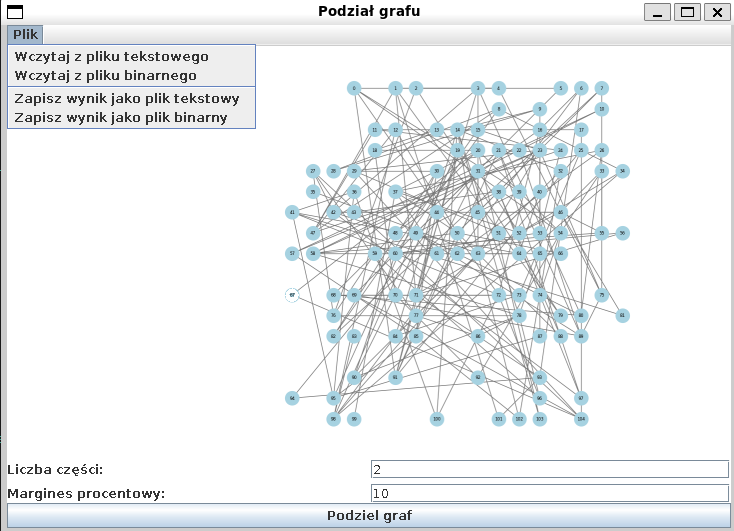
\includegraphics[width=0.9\linewidth]{img/interfejs.png}
        \caption{Przykładowy interfejs}
        \label{fig:graph}
    \end{figure}



\section{Pliki wejściowe i wyjściowe}

    \subsection{Plik wejściowy (\texttt{.csrrg} / \texttt{.bin})}
    
    Wejście programu może przyjąć dwie formy:
    \begin{itemize}
        \item Plik \texttt{.csrrg} z dodatkowymi sekcjami po piątej linii, opisującymi kolejne podgrafy powstałe z podziału grafu.
        Format pliku składa się z pięciu sekcji zapisanych w kolejnych liniach:
        \begin{enumerate}
            \item Maksymalna liczba wierzchołków w dowolnym wierszu macierzy sąsiedztwa.
            \item Lista sąsiadów wszystkich wierzchołków zapisana sekwencyjnie.
            \item Wskaźniki (indeksy) na początki list sąsiedztwa dla poszczególnych wierzchołków.
            \item Lista grup wierzchołków połączonych krawędziami (reprezentacja krawędzi).
            \item Wskaźniki na początki grup węzłów z poprzedniej listy.
        \end{enumerate}
        \item Plik binarny \texttt{.bin} — binarna forma pliku \texttt{.csrrg}, mniej czytelna dla człowieka, ale szybsza w odczycie przez program.
    \end{itemize}
    
    \subsection{Plik wyjściowy (\texttt{.csrrg2} / \texttt{.bin})}

    Po przetworzeniu danych program generuje plik wyjściowy w jednym z dwóch formatów:
    \begin{itemize}
        \item \texttt{.csrrg2} — tekstowa forma pliku wyjściowego, wzorowana na formacie wejściowym .csrrg, ale zawierająca dodatkową linię nagłówkową z wynikiem działania programu.
        \item \texttt{.bin} — binarna wersja pliku tekstowego \texttt{.csrrg2}.
    \end{itemize}
    
    W pierwszej linii pliku wyjściowego zapisywany jest rezultat działania programu w formacie:
    \begin{center}
    \texttt{<wynik (S - sukces, F - porażka)> <liczba\_części> <liczba\_przecięć> <zachowany\_margines>}
    \end{center}
    Przykład:
    \begin{center}
    \texttt{S 3 2 5}
    \end{center}



\section{Przykłady użycia}

    \subsection{Wczytywanie grafu z pliku tekstowego}
    
    Aby wczytać graf z pliku tekstowego \texttt{graf.csrrg}, wybierz opcję \texttt{Wczytaj z pliku tekstowego} z paska menu. Program odczyta dane grafu, a następnie wyświetli je w głównym obszarze aplikacji.

    \subsection{Wczytywanie grafu z pliku binarnego}
    
    Aby wczytać graf z pliku binarnego \texttt{graf.bin}, wybierz opcję \texttt{Wczytaj z pliku binarnego} z paska menu. Program odczyta dane grafu w formacie binarnym i wyświetli je w głównym obszarze aplikacji.
    
    \subsection{Podział grafu na x części z marginesem y}
    
    Po załadowaniu grafu, w panelu narzędziowym ustaw liczbę części na \texttt{x} oraz margines na \texttt{y\%}. Następnie kliknij przycisk \texttt{Podziel graf}, aby rozpocząć proces podziału. Program spróbuje podzielić graf na x części, minimalizując liczbę przeciętych krawędzi, z zachowaniem określonego marginesu różnicy liczby wierzchołków.
    
    \subsection{Zapisanie wyniku do pliku wyjściowego}
    
    Po zakończeniu podziału, aby zapisać wynik do pliku tekstowego, wybierz opcję \texttt{Zapisz wynik jako plik tekstowy} z paska menu. Program zapisze dane grafu w formacie \texttt{.csrrg2}, zawierającym dodatkową linię nagłówkową z wynikiem działania programu.
    
    \subsection{Zapisanie wyniku do pliku binarnego}
    
    Po zakończeniu podziału, aby zapisać wynik do pliku binarnego, wybierz opcję \texttt{Zapisz wynik jako plik binarny} z paska menu. Program zapisze dane grafu w formacie \texttt{.bin}, co pozwoli na szybszy odczyt danych w przyszłości.



\section{Wymagania niefunkcjonalne}

    Poniżej przedstawiono kluczowe wymagania niefunkcjonalne dla aplikacji:
    
    \begin{itemize}
        \item \textbf{Wydajność:} Czas podziału grafu powinien być jak najkrótszy dla danej wielkości grafu. Dla grafów zawierających do 1000 wierzchołków, czas przetwarzania nie powinien przekraczać minuty na standardowym sprzęcie klasy PC.
        \item \textbf{Użyteczność:} Interfejs użytkownika powinien być intuicyjny i zgodny z ogólnie przyjętymi standardami projektowania GUI.
        \item \textbf{Skalowalność:} Aplikacja powinna umożliwiać obsługę grafów o różnej wielkości, od małych do dużych.
        \item \textbf{Przenośność:} Aplikacja powinna działać poprawnie na różnych systemach operacyjnych wspierających środowisko Java.
        \item \textbf{Utrzymywalność:} Kod źródłowy aplikacji powinien być czytelny i dobrze udokumentowany, aby ułatwić przyszłe modyfikacje i rozwój.
    \end{itemize}


    

\begin{thebibliography}{9}

\bibitem{youtube_video}
Leonid Zhukov, \textit{Lecture 7. Graph partitioning algorithms.}, YouTube, 24 luty 2021, Dostępny na 28 kwietnia 2025 w: \url{https://youtu.be/zZae_C2BU_4}

\end{thebibliography}



\end{document}
